\documentclass{plt}
\usepackage{bbding} % \Checkmark \XsolidBold
\usetheme{metropolis}           % Use metropolis theme


\lstset{
  language=C,
  basicstyle={\fontsize{11}{11.5}\selectfont\ttfamily\spaceskip=3pt},
} 


\title{Basic Elements of Programming Languages}
\author{Ronghui Gu}
\institute{Columbia University}
\date{Spring 2019}
\titlegraphic{
\vspace{220pt}
{\tiny $^*$ Course website: \url{https://www.cs.columbia.edu/~rgu/courses/4115/spring2019}\vspace{-5pt}}\\
{\tiny $^{**}$ These slides are borrowed from Prof. Edwards.}
}
\begin{document}

\frame{\titlepage
}

\begin{frame}[fragile]{What is a Programming Language?}

A programming language is a notation that  a person and a computer can both understand.
\begin{itemize}

\item It allows you to express what is the \textbf{task} to compute

\item It allows a computer to \textbf{execute} the computation task

\end{itemize}

\end{frame}

\part{Language Specifications}

\tikzset{
    mymodule/.style={draw, fill=white, drop shadow},
    code/.style={draw, fill=gray!15, drop shadow,minimum width=0},
    emph/.style={draw, fill=mBlue!15, drop shadow},
    box/.style={draw, fill=white, minimum height=20, minimum width=60, drop shadow},
}

\begin{frame}[fragile]{How to Define a Language}

When designing a language, it's a good idea to start by sketching forms that you want to appear in your language as well as forms you do not want to appear.

\vspace{20pt}

\begin{minipage}{0.5\textwidth}
\begin{C}
int avg(int a, int b)
{
  return (a + b) / 2;
}
\end{C}
Examples
\end{minipage}\hspace{10pt}
\begin{minipage}{0.4\textwidth}
\begin{C}
a int vg(int a,
{
  return (a; + b) 
{ {
\end{C}
Non-Examples
\end{minipage}


\end{frame}

\begin{frame}[fragile]{How to Define a Language}

\begin{itemize}

\item An official documents, with \textbf{informal} descriptions.

\item An official documents, with \textbf{formal} descriptions.

\item A reference implementation, e.g., a compiler.
\end{itemize}
Some language definitions are sanctioned by an official standards organization, e.g.,
C11 (ISO/IEC 9899:2011).

\begin{center}
\begin{C}
int compare()
{
  int a[10], b[10]; 
  if (a > b)
    return true;
  return false;
}
\end{C}
\end{center}
\end{frame}


\begin{frame}[fragile]{Aspects of Language Specifications}

\begin{center}
\begin{tikzpicture}
  \node [box] at (0pc,0) {Syntax};
  \node [box] at (7pc,0pc) {Semantics};
  \node [box] at (14pc,0pc) {Pragmatics};
\end{tikzpicture}
\end{center}

\begin{itemize}

\item \textbf{Syntax}: how characters combine to form a program.

\item \textbf{Semantics}: what the program \emph{means}.

\item \textbf{Pragmatics}: common programming idioms; programming environments;
the standard library; ecosystems.

\end{itemize}


\end{frame}


\begin{frame}{Syntax}

Syntax is divided into:
\begin{itemize}
\item  \textbf{Microsyntax}: specifies how the characters in the source code stream are grouped into tokens.
\item \textbf{Abstract syntax}: specifies how the tokens are grouped into phrases, e.g., expressions, statements, etc.
\end{itemize}

\end{frame}

%%%%%%%%%%%%%%%%%%%%%%%%%%%%%%
\newsavebox{\gcdbox}
\begin{lrbox}{\gcdbox}
\begin{minipage}{0.4\textwidth}
\begin{C}
int avg(int a, int b)
{
  return (a + b) / 2;
}
\end{C}
\end{minipage}
\end{lrbox}
%%%%%%%%%%%%%%%%%%%%%%%%%%%%%%



\begin{frame}[fragile]{Microsytax}

Source program is just a sequence of characters.
\vspace{10pt}

\usebox{\gcdbox}

\begin{verbatim}
i  n  t SP  a  v  g  (  i  n  t SP  a  , SP  i n  t SP  b  ) NL
{ NL 
SP SP r  e  t  u  r  n SP  ( a SP + SP b ) SP / SP 2 ; NL
} NL
\end{verbatim}


\end{frame}


%%%%%%%%%%%%%%%%%%%%%%%%%%%%%%

\newcommand{\token}[1]{\tikz \node [minimum height=15pt,draw,rounded corners=2pt,fill=mBlue!10] {#1};}

\def\tokens #1 #2 #3 #4 #5 #6 #7 #8
{\token{#1} 
\token{#2} 
\token{#3} 
\token{#4}
\token{#5} 
\token{#6} 
\token{#7} 
\token{#8}
}


\begin{frame}[fragile]{Microsytax}
\usebox{\gcdbox}\hfill
%\includegraphics[width=0.45\textwidth]{subway-tokens.jpg}

\renewcommand{\baselinestretch}{1}

\vspace{5pt}

\begin{small}
\begin{tabular}{lll}
\hline
\textbf{Token} & \textbf{Lexemes} & \textbf{Pattern (as \alert{regular expressions})} \\
\hline
ID & avg, a, b & letter followed by letters or digits \\
KEYWORD & int, return & letters \\
NUMBER & 2 & digits \\
OPERATOR & +, / & +, /  \\
PUNCTUATION & ;,(,),\{,\}, & ;,(,),\{,\},  \\
\hline 
\end{tabular}
\end{small}

\vspace{5pt}

\renewcommand{\baselinestretch}{2}

{\ttfamily
\tokens int avg ( int a , int b
\tokens ) \{ return ( a + b )
\token{/} \token{2} 
\token{;} \token{\}}\par
}

\end{frame}



\begin{frame}[fragile]{Lexical Analysis Gives Tokens}
\usebox{\gcdbox}\hfill
%\includegraphics[width=0.45\textwidth]{subway-tokens.jpg}

\renewcommand{\baselinestretch}{2}

{\ttfamily
\tokens int avg ( int a , int b
\tokens ) \{ return ( a + b )
\token{/} \token{2} 
\token{;} \token{\}}\par
}

\renewcommand{\baselinestretch}{1}

\begin{itemize}
\item Throw errors when failing to create tokens:  malformed numbers (e.g., \alert{23f465\#g}) or 
invalid characters (such as \alert{non-ASCII characters} in C).
\end{itemize}

\end{frame}


\newcommand{\id}[1]{
  node [fill=gray!15] {#1}
}

\begin{frame}[fragile,t]{Abstract Syntax}

Abstract Syntax can be defined using \alert{Context Free Grammar}.

\begin{ocamlyacc}
expr :
    expr OPERATOR expr  
  | ( expr )
  | NUMBER          
\end{ocamlyacc}

Expression $ (a + b) / 2$ can be parsed into an \alert{AST}:
\begin{center}
\begin{tikzpicture}
\node {/} [level distance=2pc,
    level 2/.style={sibling distance=4.5pc},
  ]
      	child {
      		node {+}
      		child {\id a}
      		child {\id b}
      	}
      	child {node {2}}
  ;
\end{tikzpicture}
\end{center}
\end{frame}

\begin{frame}[fragile,t]{Abstract Syntax}

Abstract Syntax can be defined using \alert{Context Free Grammar}.

\begin{ocamlyacc}
expr :
    expr OPERATOR expr  
  | ( expr )
  | NUMBER          
\end{ocamlyacc}

\alert{Ambiguous!} What about $ a + b / 2$ ?

\begin{center}
\begin{minipage}{0.3\textwidth}
\begin{tikzpicture}
\node {/} [level distance=2pc,
    level 2/.style={sibling distance=4.5pc},
  ]
      	child {
      		node {+}
      		child {\id a}
      		child {\id b}
      	}
      	child {node {2}}
  ;
\end{tikzpicture}
\end{minipage}\hspace{20pt}
\begin{minipage}{0.3\textwidth}
\begin{tikzpicture}
\node {+} [level distance=2pc,
    level 2/.style={sibling distance=4.5pc},
  ]
      	child {node {a}}
      	child {
      		node {/}
      		child {\id b}
      		child {\id 2}
      	}
  ;
\end{tikzpicture}
\end{minipage}
\end{center}
\end{frame}

\newcommand{\theast}{
  \node {func} [level distance=2pc,
    level 1/.style={sibling distance=3.5pc},
    level 2/.style={sibling distance=4.5pc},
    level 3/.style={sibling distance=2.5pc},
    level 4/.style={sibling distance=2.5pc},
    level 5/.style={sibling distance=1.5pc},
  ]
  child {node {int}}
  child {node {avg}}
  child {node {args}
    child {node {arg}
      child {node {int}}
      child {\id a}}
    child {node {arg}
      child {node {int}}
      child {\id b}}
  }
  child [missing]
  child {node {return}
      child {
      	node {/}
      	child {
      		node {+}
      		child {\id a}
      		child {\id b}
      	}
      	child {node {2}}
      }
  }
  ;
}

\begin{frame}
  \frametitle{Syntax Analysis Gives an Abstract Syntax Tree}


\begin{tikzpicture}
  \theast
\end{tikzpicture}

%\vspace{-pc}
\usebox{\gcdbox}
\hspace{10pt}
\begin{minipage}{0.55\textwidth}
\begin{itemize}
\item Syntax analysis will throw errors if ``\}'' is missing. Lexical analysis will not. 
\end{itemize}
\end{minipage}

\end{frame}

\renewcommand{\id}[1]{
  node [fill=gray!15] (id) {#1}
  (id) .. controls +(-1,-2) and +(1,0) .. (#1.east)
}




\begin{frame}{Semantics}

\begin{itemize}
\item  \textbf{Static Semantics}:  deals with legality rules---things you can check \alert{before} running the code (compile time), e.g., type, scope, for some languages.
\item \textbf{Dynamic Semantics}: deals with the execution behavior; things that can only be known \alert{at} runtime, e.g., value.
\end{itemize}

\end{frame}

\begin{frame}{Static Semantics}

We can use inference rules to define semantics, e.g., type:

$$
\frac{}{\text{NUMBER}\ :\ \textbf{int}} \qquad\qquad
\frac{\text{expr}\ :\ \textbf{int}}{\text{(expr)}\ :\ \textbf{int}}
$$

$$
\frac{\text{expr}_1\ :\ \textbf{int} \quad \text{expr}_2\ :\ \textbf{int}}
{\text{expr}_1\ \text{OPERATOR}\ \text{expr}_2\ :\ \textbf{int}}
$$

\end{frame}


\begin{frame}
  \frametitle{Semantic Analysis: Resolve Symbols; Verify Types}

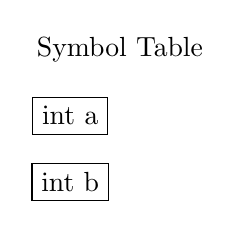
\begin{tikzpicture}
  \node at (-7.5pc, -8pc) {Symbol Table};
  \node [draw] at (-9pc,-10pc) (a) {int a};
  \node [draw] at (-9pc,-12pc) (b) {int b};
  \theast
\end{tikzpicture}

\end{frame}

\begin{frame}{Dynamic Semantics}

We can use inference rules to define semantics, e.g., value:

$$
\frac{}{\textbf{eval}\text{(NUMBER)} = \text{NUMBER}} \qquad\qquad
\frac{\textbf{eval}\text{(expr)} = n}{\textbf{eval}\text{((expr))} = n}
$$

$$
\frac{\textbf{eval}(\text{expr}_1) = n_1 \quad \textbf{eval}(\text{expr}_2) = n_2
\quad (n_1 + n _2) = n}
{\textbf{eval}(\text{expr}_1\ +\ \text{expr}_2) = n}
$$

\end{frame}

\begin{frame}{Dynamic Semantics}

Consider the integer range:

$$
\frac{\text{\alert{wrap}(NUMBER)} = n}{\textbf{eval}\text{(NUMBER)} = n} \qquad\qquad
\frac{\textbf{eval}\text{(expr)} = n}{\textbf{eval}\text{((expr))} = n}
$$

$$
\frac{\textbf{eval}(\text{expr}_1) = n_1 \quad \textbf{eval}(\text{expr}_2) = n_2
\quad \text{\alert{wrap}}(n_1 + n _2) = n}
{\textbf{eval}(\text{expr}_1\ +\ \text{expr}_2) = n}
$$

\end{frame}

\part{Programming Paradigms}

\begin{frame}{Programming Paradigms}
A programming paradigm is a \alert{style}, or ``way,'' of programming. 
Some languages make it easy to write in some paradigms but not others.
\end{frame}

%%%%%%%%%%%%%%%%%%%%%%%%%%%%%%

\begin{frame}[fragile]
  \frametitle{Imperative Programming}
An imperative program specifies \alert{how} a computation is to be done: 
a sequence of statements that update state.

\lstset{
  language=assembly,
  morekeywords={goto,return},
  basicstyle={\fontsize{8}{8.5}\selectfont\ttfamily\spaceskip=3pt},
  keywordstyle=\color{mBlue},       % keyword style
} 

\begin{assembly}
    result = []
    i = 0
    numStu = length(students)
start:
    if i >= numStu goto finished
    name = students[i]
    nameLength = length(name)
    if nameLength <= 5 goto nextOne
    addToList(result, name)
nextOne:
    i = i + 1
    goto start
finished:
    return result
\end{assembly}
\end{frame}


\begin{frame}[fragile]
  \frametitle{Structured Programming}
Programming with clean, \alert{goto-free}, nested control structures.
\href{https://homepages.cwi.nl/~storm/teaching/reader/Dijkstra68.pdf}
{\alert{Go To Statement Considered Harmful}} by Dijkstra.

\lstset{
  language=assembly,
  morekeywords={goto,return},
  basicstyle={\fontsize{8}{8.5}\selectfont\ttfamily\spaceskip=3pt},
  keywordstyle=\color{mBlue},       % keyword style
} 

\begin{assembly}
    result = []
    i = 0
    numStu = length(students)
start:
    if i >= numStu goto finished
    name = students[i]
    nameLength = length(name)
    if nameLength <= 5 goto nextOne
    addToList(result, name)
nextOne:
    i = i + 1
    goto start
finished:
    return result
\end{assembly}
\end{frame}


\begin{frame}[fragile,t]{Optimization}

\begin{center}
\hspace{20pt}
\begin{tikzpicture}
  \matrix [matrix of nodes,
           row sep=0.8pc,
           column sep=2pc,
           every node/.style={draw, fill=white, drop shadow,minimum width=5.5cm}] {
     |[code] (b)| int avg (int a, int b) ... \\
     |(a)| Lexical Analysis \\
     | (aa)| Syntax  Analysis \\
     | (aaa)| Semantic Analysis \\
     |(a4)| Intermediate Code Generation \\
     |[emph](a5)| Optimization \\
     |(a6)| Code Generation \\
    |[code] (c)| 0101110101... \\
  };
  \begin{scope}[->]
    \draw (b) -- (a);
    \draw (a) -- (aa);
    \draw (aa) -- (aaa);
    \draw (aaa) -- (a4);
    \draw (a4) -- (a5);
    \draw (a5) -- (a6);
    \draw (a6) -- (c);
  \end{scope};
  \begin{scope}[densely dotted]
    \draw (-10pc,-2.6pc) -- (10pc,-2.6pc);
    \draw (-10pc,-5pc) -- (10pc,-5pc);
  \end{scope};
  \node at (9pc,0) {front-end};
  \node at (9.5pc,-4pc) {middle-end};
  \node at (9pc,-6pc) {back-end};
\end{tikzpicture}
\end{center}

\end{frame}


\begin{frame}[fragile]
  \frametitle{Optimization}


\begin{center}
\begin{tikzpicture}
  \matrix [matrix of nodes,
           row sep=0.8pc,
           column sep=2pc,
           every node/.style={draw, fill=white, drop shadow,minimum width=5.5cm}] {
     |[emph](a)| Optimization \\
  };
  \begin{scope}[->]
    \draw (0pc,2.5pc) -- (a);
    \draw (a) -- (0pc,-2.4pc) ;
  \end{scope};
  \node at (0pc,2.5) {\begin{assembly}
avg: 
  t0 := a + b
  t1 := 2
  t2 := t0 / t1
  ret t2	
\end{assembly}};
  \node at (0pc,-5pc) {\begin{assembly}
avg: 
  t0 := a + b
  t2 := t0 / 2
  ret t2	
\end{assembly}};
\end{tikzpicture}
\end{center}

% Generated from SUIF/MachSUIF:
%
% c2s gcd.c
% do_lower gcd.suif gcd.lsuif
% do_s2m gcd.lsuif gcd.suifvm
% do_print gcd.suifvm
%
% Heavily massaged to make it readable

\end{frame}


\begin{frame}[fragile,t]{Code Generation}

\begin{center}
\hspace{20pt}
\begin{tikzpicture}
  \matrix [matrix of nodes,
           row sep=0.8pc,
           column sep=2pc,
           every node/.style={draw, fill=white, drop shadow,minimum width=5.5cm}] {
     |[code] (b)| int avg (int a, int b) ... \\
     |(a)| Lexical Analysis \\
     | (aa)| Syntax  Analysis \\
     | (aaa)| Semantic Analysis \\
     |(a4)| Intermediate Code Generation \\
     |(a5)| Optimization \\
     |[emph] (a6)| Code Generation \\
    |[code] (c)| 0101110101... \\
  };
  \begin{scope}[->]
    \draw (b) -- (a);
    \draw (a) -- (aa);
    \draw (aa) -- (aaa);
    \draw (aaa) -- (a4);
    \draw (a4) -- (a5);
    \draw (a5) -- (a6);
    \draw (a6) -- (c);
  \end{scope};
  \begin{scope}[densely dotted]
    \draw (-10pc,-2.6pc) -- (10pc,-2.6pc);
    \draw (-10pc,-5pc) -- (10pc,-5pc);
  \end{scope};
  \node at (9pc,0) {front-end};
  \node at (9.5pc,-4pc) {middle-end};
  \node at (9pc,-6pc) {back-end};
\end{tikzpicture}
\end{center}

\end{frame}
%%%%%%%%%%%%%%%%%%%%%%%%%%%%%%

\begin{frame}[fragile]{Generation of x86 Assembly}


\begin{center}
\begin{tikzpicture}
  \matrix [matrix of nodes,
           row sep=0.8pc,
           column sep=2pc,
           every node/.style={draw, fill=white, drop shadow,minimum width=5.5cm}] {
     |[emph](a)| Code Generation \\
  };
  \begin{scope}[->]
    \draw (0pc,2.5pc) -- (a);
    \draw (a) -- (0pc,-1.5pc) ;
  \end{scope};
  \node at (0pc,1.7) {\begin{assembly}
avg: 
  t0 := a + b
  t2 := t0 / 2
  ret t2	
\end{assembly}};
  \node at (0pc,-6.5pc) {\begin{assembly}
avg:  pushl %ebp          # save BP
      movl  %esp,%ebp
      movl  8(%ebp),%eax  # load a from stack
      movl  12(%ebp),%edx # load b from stack
      
      addl  %edx,%eax     # a += b
      shr   $1,%eax       # a /= 2
      ret
\end{assembly}};
\end{tikzpicture}
\end{center}


%\raisebox{2pc}{\scalebox{0.75}{\usebox{\gcdbox}}}\hfill \includegraphics[width=5pc]{80386.jpg}


\end{frame}

\end{document}

% Local Variables:
% compile-command: "make processors.pdf"
% End:

